% limen-guide.tex -- руководство к пакету limen, оформленное им самим.
% Сборка из корня проекта: make doc. Или здесь же, если limen виден TeX: lualatex limen-guide.tex, трижды.
\documentclass[10pt,a4paper]{article}
\usepackage[a4paper,left=58mm,right=17mm,top=30mm,bottom=29mm,headsep=8mm,footskip=11mm]{geometry}
\usepackage{fontspec}
\makeatletter
\ifdefined\l@russian\else
  \newlanguage\l@russian
  \directlua{
    local function slurp(n) local f = assert(io.open(n, "r")) local s = f:read("*a") f:close() return s end
    local l = lang.new(\the\l@russian)
    lang.patterns(l, slurp("hyph-ru.pat.txt"))
    lang.hyphenation(l, slurp("hyph-ru.hyp.txt"))}
\fi
\makeatother
\usepackage[provide=*]{babel}
\babelprovide[import,main,hyphenrules=russian]{russian}
\lefthyphenmin=2 \righthyphenmin=2
\newcommand\curvesep{,}
% limen-guide-common.tex -- the layout shared by the guides. The guides load fontspec and their language first.
\setmainfont{Lora}[Path=../doc/fonts/,Extension=.ttf,UprightFont=*-Regular,BoldFont=*-Bold,
  ItalicFont=*-Italic,BoldItalicFont=*-BoldItalic,Ligatures=TeX]
\setsansfont{Inter}[Path=../doc/fonts/,Extension=.otf,UprightFont=*-Regular,BoldFont=*-SemiBold,
  ItalicFont=*-Italic,BoldItalicFont=*-Bold,Scale=0.9]
\linespread{1.1}
\usepackage{microtype}
\usepackage{fancyhdr,booktabs,tabularx,array,enumitem,caption,graphicx,fancyvrb,tikz}
\usepackage[hidelinks]{hyperref}
\usepackage[palette=ultramarine]{limen}
\limensetup{initialfont=fonts/Lora-Bold.ttf}
\graphicspath{{../gallery/}{gallery/}}
\definecolor{textc}{HTML}{1E1D22}
\definecolor{muted}{HTML}{5C5A63}
\definecolor{rulec}{HTML}{D6D3DE}
% chart colours, checked for separation under colour blindness and for contrast on the page
\definecolor{chartA}{HTML}{3D57C7}
\definecolor{chartB}{HTML}{B47A12}
\color{textc}
\hypersetup{colorlinks=true,linkcolor=limenink,urlcolor=limenink}
\makeatletter
\renewcommand\section{\@startsection{section}{1}{\z@}{-2.8ex plus -.6ex minus -.2ex}{1.2ex plus .2ex}%
  {\normalfont\large\bfseries\color{limenink}}}
\renewcommand\subsection{\@startsection{subsection}{2}{\z@}{-2ex plus -.4ex minus -.2ex}{.7ex plus .1ex}%
  {\normalfont\normalsize\bfseries\color{limenink}}}
\renewcommand\l@section{\@dottedtocline{1}{0pt}{1.6em}}
\renewcommand\numberline[1]{\hb@xt@\@tempdima{#1\hfil}}
\makeatother
\setcounter{secnumdepth}{1}
\setcounter{tocdepth}{1}
\pagestyle{fancy}\fancyhf{}\renewcommand\headrulewidth{0pt}
\fancyfoot[R]{\footnotesize\sffamily\color{muted}\thepage}
\setlist{leftmargin=1.2em,itemsep=2pt,topsep=3pt,parsep=0pt}
\setlist[itemize]{label={\color{limenaccent}\textbullet}}
\captionsetup{font={footnotesize,sf},labelfont=bf,labelsep=period,justification=raggedright,singlelinecheck=false,skip=5pt}
\setlength\parindent{0pt}\setlength\parskip{.55em plus .1em}
\emergencystretch=3em
\providecommand\curvesep{.}
% commands and options in the text
\newcommand\cs[1]{\texttt{\textbackslash #1}}
\newcommand\opt[1]{\texttt{#1}}
% tables
\newcolumntype{L}{>{\raggedright\arraybackslash\sffamily\footnotesize}X}
\newcolumntype{P}[1]{>{\raggedright\arraybackslash\sffamily\footnotesize}p{#1}}
\newcolumntype{T}[1]{>{\raggedright\arraybackslash\ttfamily\footnotesize}p{#1}}
\newcommand\thead[1]{\textbf{\sffamily\footnotesize #1}}
\newcommand\fig[3][1]{\par\medskip\noindent\begin{minipage}{\linewidth}\includegraphics[width=#1\linewidth]{#2}\captionof{figure}{#3}\end{minipage}\par\medskip}
\DefineVerbatimEnvironment{code}{Verbatim}{fontsize=\small,formatcom=\color{limenink},xleftmargin=.6em,samepage=true}
% the curve of the story, computed by the package itself; #1 lists thresholds as shares of the document
\newcommand\curvepts[1]{\directlua{
  local Art = require("limen-art")
  local ths = {}
  for v in string.gmatch("#1", "[0-9.]+") do table.insert(ths, { i = tonumber(v) * 100 + 1, y = 1 }) end
  local S = Art.make_story(1, 1, Art.defaults(), { pages = 100, ths = ths })
  local t = {}
  for k = 0, 200 do table.insert(t, "(" .. k / 200 .. "," .. S.curve(k / 200, 0.04, 0.07) .. ")") end
  tex.sprint(table.concat(t, " -- "))}}
% #1 x label, #2 y label, #3 legend of one threshold, #4 legend of three, #5 caption
\newcommand\curvefig[5]{\par\medskip\noindent\begin{minipage}{\linewidth}\centering
  \begin{tikzpicture}[x=.88\linewidth,y=34mm,font=\sffamily\footnotesize]
    \foreach \v/\t in {0/0,.5/0\curvesep 5,1/1} {\draw[rulec,line width=.3pt] (0,\v) -- (1,\v); \node[anchor=east,text=muted] at (0,\v) {\t};}
    \foreach \v/\t in {0/0,.25/0\curvesep 25,.5/0\curvesep 5,.75/0\curvesep 75,1/1} {\draw[rulec,line width=.3pt] (\v,0) -- (\v,-.03); \node[anchor=north,text=muted] at (\v,-.03) {\t};}
    \edef\limentmp{\noexpand\draw[chartB,line width=1.3pt,line join=round] \curvepts{0.18,0.5,0.75};}\limentmp
    \edef\limentmp{\noexpand\draw[chartA,line width=1.3pt,line join=round] \curvepts{0.25};}\limentmp
    \node[anchor=north,text=muted] at (.5,-.14) {#1};
    \node[anchor=south,rotate=90,text=muted] at (-.07,.5) {#2};
    \draw[chartA,line width=1.3pt] (0,1.13) -- (.05,1.13); \node[anchor=west] at (.05,1.13) {#3};
    \draw[chartB,line width=1.3pt] (.42,1.13) -- (.47,1.13); \node[anchor=west] at (.47,1.13) {#4};
  \end{tikzpicture}
  \captionof{figure}{#5}\end{minipage}\par\medskip}

\hypersetup{pdftitle={limen: руководство},pdflang={ru}}
\fancyhead[R]{\footnotesize\sffamily\color{muted}limen: руководство}

\begin{document}
\limencover{limen}{Поля страницы, где свет заслуживает цвет}{Руководство к версии 0.2\\Ноябрь 2026}

\limeninitial{L}imen (лат.\ «порог») это пакет для LuaLaTeX, который рисует на полях ночное поле, тонкие линии равной фазы и луч. У каждого заголовка луч сходится в белую звезду, а между заголовками раскладывается в спектр. Всё считается на Lua в момент вывода страницы и записывается прямо в PDF: ни картинок, ни внешних файлов.

Главное в нём не рисунок, а сюжет. На первых страницах луч тонкий и почти белый, поле тёмное, линии только проступают. На пороге начинается рост, и к концу документа полный спектр уходит за край листа. Документ получает развитие, которое видно, даже если просто листать его. Посмотреть, как это работает, можно на этом руководстве: оно оформлено самим пакетом.

\fig{story.png}{Поля восьмистраничного документа подряд: ниже порога, порог, рост, финал.}

\begingroup\small\setlength\parskip{0pt}\tableofcontents\endgroup

\section{Когда применять}

Стиль яркий и сильно влияет на то, как воспринимается документ. Он подходит не для всего. Вот как решать.

\medskip
\noindent\begin{tabularx}{\linewidth}{@{}P{42mm}L@{}}
\toprule
\thead{Подходит} & \thead{Почему}\\\midrule
Тексты про свет, лазеры, оптику, спектроскопию, излучение & Образ связан с темой, а не приклеен к ней\\
Разборы, отчёты лаборатории, научно-популярные тексты, раздаточные материалы & Читают по своей воле, и оформление помогает выделить документ\\
Документы с поворотом: «сначала казалось так, а на самом деле иначе» & Порог ставится прямо на поворот, и рисунок работает на мысль\\
Чтение с экрана, от 3 до 40 страниц & Сюжету нужно место, а тёмным полям не нужна печать\\
Доклады и семинары & Слайдов обычно 10–30, и рост хорошо виден при показе\\
\bottomrule
\end{tabularx}

\medskip
\noindent\begin{tabularx}{\linewidth}{@{}P{42mm}L@{}}
\toprule
\thead{Лучше не применять} & \thead{Что вместо}\\\midrule
Подача в журнал, ГОСТ, договоры, официальные бланки & Оформление там задано правилами. Используйте шаблон издания\\
Офисная печать в тёмном режиме & Режим \opt{mode=paper}: светлое поле расходует гораздо меньше краски\\
Одна-две страницы & Сюжету негде развернуться. Подойдёт \opt{story=flat}\\
Широкие таблицы и рисунки на каждой странице & Колонка занимает около 5~см. Выделите широкие страницы, см.\ раздел~\ref{recipes}, или откажитесь от пакета\\
Длинные книги & Один рост на сотни страниц незаметен. Подойдёт \opt{story=chapter}\\
Темы, не связанные со светом & Образ окажется случайным, а читатель будет искать в нём смысл\\
Текст, который видят с одной открытой страницы & Первые страницы намеренно сдержанны. Передвиньте порог ближе к началу\\
Читателю мешает радуга, а луч важен & Режим \opt{beam=mono}: один цвет, как у настоящего лазера\\
\bottomrule
\end{tabularx}

\section{Как начать}

Нужен LuaLaTeX и LaTeX не старше октября 2020 года. Проверялись выпуски 2023 и 2026 годов, см.\ раздел~\ref{checked}. С pdfLaTeX и XeLaTeX пакет не работает, потому что весь рисунок считается на Lua.

Установка: положите рядом с документом файлы \opt{limen.sty}, \opt{limen.lua}, \opt{limen-art.lua}, \opt{limen-pdf.lua} и \opt{limen-palettes.lua}. Чтобы пакет был виден всем документам, выполните \opt{make install}.

\begin{code}
\documentclass[10pt,a4paper]{article}
\usepackage[left=58mm,right=17mm,top=30mm,bottom=29mm]{geometry}
\usepackage[palette=ultramarine]{limen}
\begin{document}
\section{Below the threshold}
...
\end{document}
\end{code}

Собирать нужно два раза, как при оглавлении, потому что сюжету нужна длина документа. Команда \opt{latexmk -lualatex} делает нужное число проходов сама. Если длина изменилась, пакет напишет в журнале, что нужен ещё проход.

Работа с пакетом обычно сводится к трём шагам.
\begin{enumerate}[leftmargin=1.5em]
\item \textbf{Освободить поле.} Рисунок занимает левое поле целиком. Для А4 хорошо работает 58~мм. Если колонка окажется уже 2,5~см, пакет предупредит.
\item \textbf{Выбрать палитру.} Обычно по лазеру или теме, см.\ раздел~\ref{palettes}.
\item \textbf{Поставить порог.} Команда \cs{limenthreshold} на повороте мысли. Если поворота нет, порог останется на 25~\% документа.
\end{enumerate}
Заголовки, рост и финал пакет расставляет сам. Текст и его разбивка на страницы от рисунка не зависят: это проверяется тестами.

\section{Сюжет}
\limenthreshold

Порог этого руководства стоит прямо у заголовка «Сюжет». Посмотрите на левое поле: до этого места луч был белым, а отсюда начинается цвет.

Кривая устроена как зависимость мощности лазера от накачки: ниже порога почти ничего, выше него почти прямая. Если порогов несколько, рост идёт ступенями: каждый порог начинает подъём, который успевает затихнуть до следующего.

\curvefig{Доля документа}{Раскрытие спектра}{Один порог, 0,25}{Три порога: 0,18, 0,5 и 0,75}{Как раскрывается спектр по ходу документа. Кривые посчитаны тем же кодом, что рисует поля.}

По этой кривой растут ширина спектра, цвет поля, яркость линий и каустик, размер звёзд. Рост непрерывный и внутри страницы, поэтому порог виден как событие на конкретном листе, а не как скачок между листами.

\begin{itemize}
\item \cs{limenthreshold} ставит порог в это место текста. Звезда здесь крупнее остальных. Несколько таких команд дают ступени.
\item \opt{threshold=0.1} задаёт порог долей документа, если места поворота нет.
\item \opt{story=flat,level=0.7} отключает рост и держит одну стадию, для коротких текстов.
\item \opt{story=chapter} запускает сюжет заново в каждой главе. В классах без глав то же делает \cs{limenrestart}.
\item \cs{limenlevel\{0.9\}} задаёт стадию вручную со страницы, где стоит. Пустое \cs{limenlevel\{\}} возвращает обычный ход.
\item \cs{limenend} завершает сюжет раньше, например перед приложениями. Без него финал на последней странице.
\end{itemize}

Звезда всегда означает заголовок или метку в тексте. На длинном участке без заголовков луч просто сужается, а если звезда там нужна, её ставит \cs{limenstar}.

Если на странице финала остаётся много места, ночное поле разливается под текстом, а луч проходит большую каустику и уходит веером за правый край. Номер страницы там становится белым сам, с любым стилем страницы. Если места мало, веер получается небольшим и уходит через левое поле.

\section{Опции}

Опции задаются при загрузке пакета или в преамбуле через \cs{limensetup\{...\}}.

\medskip
\noindent\begin{tabularx}{\linewidth}{@{}T{26mm}P{33mm}L@{}}
\toprule
\thead{Опция} & \thead{Значения} & \thead{Что делает}\\\midrule
palette & см.\ раздел~\ref{palettes} & Цвета поля, линий и заголовков\\
mode & night, paper & Тёмное поле для экрана или светлое для принтера\\
story & threshold, flat, chapter & Один рост, одна стадия или рост в каждой главе\\
threshold & 0--0.9, обычно 0.25 & Где порог, если нет \cs{limenthreshold}\\
level & 0--1, обычно 0.75 & Стадия при \opt{story=flat}\\
beam & spectrum, mono & Радуга или один цвет, как у настоящего лазера\\
wavelength & нм & Длина волны при \opt{beam=mono}. Обычно своя у палитры\\
caustic & ellipse, cardioid, nephroid, rings, speckle, mix & Вид каустик\\
caustics & 0, 1, 2 & Сколько каустик на странице, не больше\\
density & 0.2--3, обычно 1 & Сколько линий равной фазы\\
lines & true, false & Линии равной фазы\\
headings & true, false & Звёзды у заголовков\\
finale & true, false & Финальный веер\\
headrule & true, false & Линейка над текстом\\
column & см & Ширина цветной колонки. Обычно она доходит до текста\\
seed & число & Другой рисунок при том же сюжете\\
paper & цвет HTML & Цвет бумаги, если он не белый, вместе с \cs{pagecolor}\\
initialfont & auto, файл & Шрифт буквицы. Обычно это полужирное начертание документа\\
color & rgb, cmyk & Цветовая модель рисунка, см.\ раздел~\ref{paper}\\
bleed & мм & Выпуск за обрез на каждую сторону, см.\ раздел~\ref{paper}\\
sameart & true, false & Один рисунок на всех страницах, для анимации\\
draft & & Без рисунка: быстрая сборка на время правки текста\\
\bottomrule
\end{tabularx}

\section{Команды}

\medskip
\noindent\begin{tabularx}{\linewidth}{@{}T{52mm}L@{}}
\toprule
\thead{Команда} & \thead{Что делает}\\\midrule
\textbackslash limenthreshold & Порог в этом месте текста\\
\textbackslash limenstar & Звезда на луче у этой строки\\
\textbackslash limencaustic[kind=rings,size=1.3] & Каустика у этой строки: вид и радиус в сантиметрах\\
\textbackslash limenrestart & Новый сюжет при \opt{story=chapter}\\
\textbackslash limenlevel\{0.9\} & Стадия вручную, начиная с этой страницы\\
\textbackslash limenpause & На этой странице рисунка нет\\
\textbackslash limenoff, \textbackslash limenon & Выключить и снова включить рисунок\\
\textbackslash limenend & Финал здесь, а не на последней странице\\
\textbackslash limeninitial[3]\{T\}his & Буквица высотой в три строки. Текст копируется и ищется целым словом\\
\textbackslash limenrule[0.5\textbackslash linewidth] & Разделитель: тонкое веретено спектра\\
\textbackslash limenspark[0.8em] & Блик размером с букву\\
\textbackslash limenspectrum[4cm] & Полоска спектра от 400 до 700~нм\\
\textbackslash limencover[style=dark]\{\}\{\}\{\} & Обложка: заголовок, подзаголовок, подробности\\
\textbackslash limendefinepalette\{name\}\{...\} & Своя палитра, в преамбуле\\
\textbackslash limensetup\{...\} & Изменить опции, в преамбуле\\
\bottomrule
\end{tabularx}

\medskip
В тексте доступны цвета \opt{limenink} и \opt{limenaccent}. Если задать ими заголовки и маркеры, текст совпадёт по цвету с полями.

\section{Палитры, луч и каустики}\label{palettes}

\fig{palettes.png}{Слева направо: ultramarine, peacock, ruby, emerald, infrared, graphite. Показан финал.}

\begin{itemize}
\item \opt{ultramarine}. Основная: синяя ночь и золотые линии. Подходит почти всегда, и радуга на ней видна лучше всего.
\item \opt{peacock}. Бирюза и изумруд. Мягче, но цвет поля отчасти спорит с лучом.
\item \opt{ruby}. Рубиновый лазер, 694~нм. Тёплая и драматичная.
\item \opt{emerald}. Вторая гармоника Nd:YAG, 532~нм.
\item \opt{infrared}. Сам Nd:YAG, 1064~нм, в цветах тепловизора.
\item \opt{graphite}. Без цвета на поле: цвет есть только у луча. Самая строгая.
\end{itemize}

Своя палитра задаётся в преамбуле. Обязательных ключей нет, недостающие берутся из \opt{ultramarine}.
\begin{code}
\limendefinepalette{dusk}{deep=1B1033, flow=5A2A7A, flow2=A83E6A,
  line=FFD9A0, caustic=FFC48A, ink=5A2A7A, accent=C9773A}
\limensetup{palette=dusk}
\end{code}
Здесь \opt{deep} это цвет ночи, \opt{flow} и \opt{flow2} это медленные потоки на ней, \opt{line} это линии, \opt{caustic} это каустики, \opt{ink} и \opt{accent} это цвета для текста. Поле должно быть тёмным: луч ярко виден только на тёмном.

\textbf{Один цвет.} С \opt{beam=mono} радуги нет: луч одного цвета, как у настоящего лазера, а сюжет виден по его ширине и накалу. Длина волны берётся из палитры или задаётся опцией \opt{wavelength}. Выше 720~нм свет невидим, поэтому цвет условный, как на тепловизоре.

\fig[.84]{mono.png}{Палитра emerald с \opt{beam=mono}: начало, рост, финал.}

\textbf{Каустики.} Опция \opt{caustic} выбирает вид для всего документа, значение \opt{mix} чередует их, а \cs{limencaustic} ставит нужную у конкретной строки.

\medskip
\noindent\begin{minipage}[c]{.2\linewidth}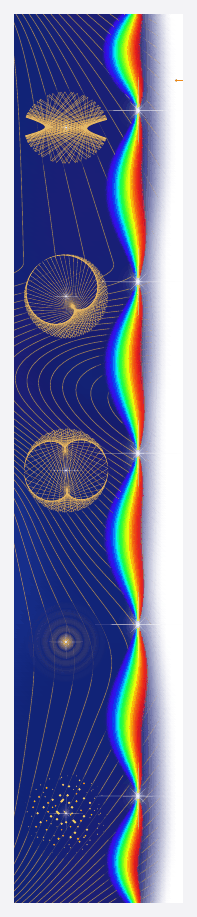
\includegraphics[width=\linewidth]{caustics.png}\end{minipage}\hfill
\begin{minipage}[c]{.76\linewidth}
\begin{itemize}
\item \opt{ellipse}. Луч внутри эллиптического зеркала. Траектории, которые почти замыкаются и дают фигуры, похожие на символы, отбрасываются.
\item \opt{cardioid}. Каустика чашки при свете от точки на её краю, та самая фигура на дне кружки.
\item \opt{nephroid}. Каустика чашки при параллельном свете.
\item \opt{rings}. Дифракция на круглом отверстии, $(2J_1(x)/x)^2$ до пятого тёмного кольца. Внешние кольца подняты по яркости, иначе их не видно.
\item \opt{speckle}. Спекл: сумма волн со случайными направлениями и фазами, золотая пыль в ярких максимумах.
\end{itemize}
\end{minipage}

\section{Печать}\label{paper}

\textbf{Обычный принтер.} В тёмном режиме поля закрывают примерно четверть листа, а обычный принтер не печатает в край. Для бумаги есть \opt{mode=paper}: то же построение на светлом фоне, тёмный луч вместо белого, а спектр появляется там же, где и в ночном режиме.

\fig[.84]{paper.png}{Тот же документ в режиме \opt{mode=paper}.}

На примере из галереи средняя темнота страницы падает с 27~\% до 7~\%. Это грубая мера, подсчитанная по рендеру, а не расход краски конкретным принтером. На настоящем принтере режим пока не проверялся.

\textbf{Типография.} Опция \opt{color=cmyk} рисует всё в DeviceCMYK, а \opt{bleed=3} добавляет 3~мм на каждую сторону листа и записывает TrimBox и BleedBox. Рисунок и обложка уходят за линию реза.
\begin{code}
\usepackage[cmyk]{xcolor}
\usepackage[color=cmyk,bleed=3]{limen}
\end{code}
Цвет пересчитывается простой формулой, без профиля ICC, и насыщенные цвета спектра в CMYK заметно тускнеют. Метки реза и PDF/X пакет не делает. Поэтому перед тиражом нужна цветопроба в типографии.

\textbf{Лист проверки.} Прежде чем печатать много, распечатайте один лист \opt{doc/limen-print-test.pdf}, он же \opt{make print-test}. На нём стадии луча в настоящем размере, один и тот же веер в RGB и CMYK, тёмные поля всех палитр, линии от 0,2 до 1~пт, плавные переходы и текст у края поля. Всё держится в 10~мм от края, так что лист помещается и на обычном принтере. Масштаб печати должен быть 100~\%.

\section{Обложка}

Команда \cs{limencover\{title\}\{subtitle\}\{details\}} занимает целую страницу. На ней сразу виден полный спектр, как обещание того, чем закончится документ. С \opt{style=dark} на обложке только белый луч, и цвет остаётся полностью на потом. Обложка не считается в сюжете, но номер страницы занимает: если нужно, задайте \cs{setcounter\{page\}\{1\}} после неё.

\section{Украшения в тексте}

Разделитель \cs{limenrule} подходит для смены темы внутри раздела:
\limenrule
Блик \limenspark{} стоит в строке как буква. Полоска \limenspectrum[3cm] удобна в подписях и легендах. Они всегда нарисованы для светлой страницы, в обоих режимах.

\section{Слайды}

Пакет сам определяет класс \opt{beamer}. Поля становятся узкой колонкой слева, оверлеи одного кадра получают один и тот же рисунок, сюжет считается по кадрам, а не по страницам PDF.

\begin{code}
\documentclass[aspectratio=169]{beamer}
\usepackage{limen}
\begin{document}
\begin{frame}[plain]\limencover{Title}{Subtitle}{Details}\end{frame}
\begin{frame}{Below the threshold} ... \end{frame}
\begin{frame}{The turn}\limenthreshold ... \end{frame}
\end{document}
\end{code}

\fig{slides.png}{Обложка, кадр ниже порога и кадр выше него.}

Ширину колонки на слайдах задавайте опцией пакета, \opt{column=2.2}, а не через \cs{limensetup}: от неё зависит отступ текста.

\section{Без LaTeX: SVG, Typst, браузер}

Рисование отделено от TeX, поэтому тот же файл \opt{limen-art.lua} работает и без него.

\textbf{SVG.} Команда рисует одну страницу. Нужен любой Lua 5.3 или новее, например \opt{texlua} из LuaTeX. Контуры остаются векторными, а поле и луч становятся картинкой PNG внутри файла, потому что в SVG нет цветовых сеток.
\begin{code}
texlua limen-svg.lua --page 3 --pages 8 --palette ruby > page-3.svg
texlua limen-svg.lua --help
\end{code}

\textbf{Typst.} Файл \opt{typst/limen.typ} оставляет метки у заголовков, а \opt{typst/build.py} читает их, рисует по SVG на страницу и собирает документ с этими рисунками на фоне. Неизменившиеся страницы заново не рисуются.
\begin{code}
#import "limen.typ": limen, limen-threshold, limen-caustic
#show: limen

python3 typst/build.py report.typ --palette ultramarine
\end{code}
Поверх рисунка в Typst идёт его собственный текст. Буквицы, обложки и украшений в тексте там пока нет.

\textbf{Браузер.} Страница \opt{web/index.html} подбирает палитру, порог, луч и каустики на примере из восьми страниц и сразу показывает результат. Рядом готовые строки для LaTeX, Typst и командной строки, а настройки хранятся в адресе, так что результат можно отправить ссылкой. Lua там работает через Fengari, примерно в 20 раз медленнее, чем в LuaTeX, поэтому показ упрощён: сетки реже, чем в готовом PDF. Кнопка копирования SVG считает страницу в полном качестве. Контуры при этом получаются те же самые, байт в байт. Сервер не нужен: страницу можно открыть из папки.

\section{Рецепты}\label{recipes}

\textbf{Широкая таблица в середине.} Рисунок следует за разметкой каждой страницы, так что достаточно изменить поля:
\begin{code}
\clearpage\newgeometry{left=32mm,right=12mm}
... the table ...
\clearpage\restoregeometry
\end{code}
Если колонка стала слишком узкой, добавьте на эту страницу \cs{limenpause}.

\textbf{Приложения и список литературы вне сюжета.} Поставьте \cs{limenend} перед ними. Финал будет там, а следующие страницы останутся на полной стадии.

\textbf{Свои заголовки.} Звёзды ставятся автоматически в заголовках стандартных классов, KOMA-Script, memoir и тегированных документов. Пакет \opt{titlesec} заменяет код заголовков, поэтому добавьте звезду в формат:
\begin{code}
\titleformat{\section}{\bfseries}{\thesection}{1em}{\limenstar}
\end{code}

\textbf{Двусторонняя печать.} С опцией класса \opt{twoside} и широким внешним полем рисунок сам переходит на внешнее поле и отражается.

\textbf{Цветная бумага.} Цвет должен быть известен и пакету, иначе край поля растворится в белом:
\begin{code}
\usepackage[paper=FBF6EA]{limen}
\pagecolor[HTML]{FBF6EA}
\end{code}

\textbf{Тегированный PDF.} Подключите теги через \cs{DocumentMetadata}, а весь рисунок пакет сам пометит как оформление (Artifact), чтобы программы чтения с экрана его пропускали. Нужен LaTeX 2024 года или новее.
\begin{code}
\DocumentMetadata{lang=ru,tagging=on}
\documentclass{article}
\end{code}

\textbf{Другой рисунок при том же сюжете.} Измените \opt{seed}. Один и тот же файл с одним зерном всегда даёт один и тот же рисунок.

\textbf{Быстрая правка.} На время работы над текстом подойдёт опция \opt{draft}. Разбивка на страницы будет той же самой.

\textbf{Ошибка cannot find file ''.} Кэш шрифтов запоминает путь, по которому шрифт загрузили первым. Если этот путь был относительным, а другой документ берёт копию того же файла с тем же размером и временем из другой папки, LuaLaTeX остановится на этой ошибке. Это особенность загрузчика шрифтов, она бывает и без limen. Помогает абсолютный \opt{Path} в \cs{setmainfont} или удаление файла этого шрифта из папки кэша \opt{luatex-cache/generic/fonts/otl}. В документе с буквицей пакет заранее предупредит об этом в журнале.

\section{Как это устроено}

\begin{itemize}
\item \textbf{Одна форма на страницу.} Весь рисунок страницы записывается в один объект PDF (Form XObject) со своими ресурсами. Так пакет не зависит от того, что делают с ресурсами страницы другие пакеты.
\item \textbf{Своя группа прозрачности.} На странице указано, в каком цветовом пространстве смешивать полупрозрачные линии и блики, чтобы это не выбирал просмотрщик.
\item \textbf{Плавные сетки вместо стопок контуров.} Цвет задан сетками с интерполяцией (PDF shading type 5). Это даёт ровный переход без ступеней при любом увеличении.
\item \textbf{Никаких режимов наложения.} Сложение света считается заранее на Lua, и в PDF попадают готовые непрозрачные цвета. Сетка с наложением Screen в Poppler становилась белой, потому что каждый треугольник накладывается отдельно.
\item \textbf{Спектр считается честно.} Луч это сумма гауссовых полос, по одной на длину волны, с постоянной энергией. Поэтому узкий луч действительно складывается в белый, а широкий действительно расходится на чистые цвета.
\item \textbf{Каустики считаются честно.} Это трассировка лучей, геометрия огибающих и формула дифракции.
\item \textbf{Финал измеряется, а не угадывается.} На последней странице реальная высота содержимого берётся из готовой страницы при выводе, поэтому плавающие рисунки и сноски учитываются, и ночное поле их не закрывает.
\item \textbf{Без зависимости от порядка таблиц Lua.} Линии обходятся в отсортированном порядке, а случайные числа не зависят от разрядности целых чисел, поэтому браузер и LuaTeX считают одно и то же.
\end{itemize}

Условность остаётся одна, и она важная: настоящий луч Nd:YAG одноцветный и невидимый (1064~нм). Радуга здесь образ, ближайшая физика это суперконтинуум. Масштаб линий и изгибы луча декоративные.

Идея рисовать поля процедурно на Lua и код поиска меток в готовой странице взяты из пакета florilegium Кевина Рэймонда (MIT). Сам рисунок, сюжет и вывод написаны заново, и florilegium для работы не нужен.

\section{Что проверено и чего нет}\label{checked}

\noindent\begin{tabularx}{\linewidth}{@{}P{26mm}L@{}}
\toprule
\thead{Проверено} & \thead{На чём}\\\midrule
Сборка & Чистый TeX Live 2026 (TinyTeX, LuaHBTeX 1.24.0, LaTeX 2026-06-01) и TeX Live 2023 (Debian, LuaHBTeX 1.17.0, LaTeX 2023-11-01, часть пакетов добавлена вручную)\\
Классы & article, report, book, scrartcl, memoir, beamer\\
Разметка & А4, А5, Letter, альбомная, две колонки, двусторонняя печать, узкое поле, смена полей посреди документа, цветная бумага\\
Содержимое & Русский язык (babel), fancyhdr, titlesec, hyperref, TikZ, плавающие рисунки и сноски на странице финала, теги \cs{DocumentMetadata} (только 2026)\\
Просмотр & Poppler 24.02, PDFium 158 (движок Chrome), pdf.js 3.2: страницы сравниваются автоматически, см.\ \opt{tools/crosscheck.py}. Adobe Acrobat на Windows: вручную просмотрены обложка, страница с рисунками и последняя страница\\
Без LaTeX & Typst 0.15.1. SVG сверен с PDF (\opt{tools/svgcheck.py}, разница до 0,6~\%). Страница в браузере проверена в Chromium\\
Тесты & 31 документ через \opt{make test}: текст с рисунком и без него совпадает слово в слово, звёзды дошли до каждого заголовка, повторная сборка даёт те же пиксели, CMYK и рамки листа на месте, предупреждения только ожидаемые\\
\bottomrule
\end{tabularx}

\medskip
\textbf{Не проверено:} Preview на macOS, Ghostscript, MuPDF, настоящая печать на принтере и в типографии, MiKTeX, Windows, macOS, PDF/A и PDF/X. Теги проверены только по содержимому файла: валидаторами PAC и veraPDF документы не прогонялись.

\textbf{Скорость и размер.} Сборка занимает около половины секунды на страницу, файл растёт примерно на 120~КБ на страницу. В просмотрщиках с Poppler (Evince, Okular) страница появляется за 1--4~с, потому что он дробит сетки на мелкие кусочки. В PDFium и pdf.js это занимает от 0,02 до 0,3~с. Acrobat при частой смене масштаба дорисовывает страницу с задержкой, и рисунки на это время могут пропадать.

\textbf{Известные ограничения.}
\begin{itemize}
\item Текст не должен заходить на левое поле: рисунок лежит под ним, и читаемость там не гарантируется.
\item В режиме двух колонок разлива на последней странице нет, остаётся небольшой веер.
\item Автоматические звёзды работают не с любым кодом заголовков. Если их нет, используйте \cs{limenstar}.
\item Звёздные заголовки (\cs{subsection*}) считаются заголовками первого уровня и получают крупную звезду.
\end{itemize}

\section{Что осталось}

\textbf{Сделать может только человек.}
\begin{itemize}
\item Открыть файлы в Preview на Mac, распечатать \opt{mode=paper} на обычном принтере. Это самый большой оставшийся риск.
\item Завести репозиторий и дождаться первого запуска сборки: файлы \opt{.github/workflows} написаны для Linux, Windows и macOS, но ещё ни разу не выполнялись.
\item Вписать имя в \opt{LICENSE} и \opt{build.lua}, проверить имя пакета на CTAN и отправить архив, собранный \opt{l3build ctan}.
\end{itemize}

\textbf{Опробовано и отклонено.} Ускорить показ в Poppler параметрическими сетками не вышло. На опытной сборке Poppler стал быстрее лишь чуть-чуть (1,3--1,7~с вместо 1,3--2,1~с на страницу), файл вырос в 3--4 раза, а pdf.js замедлился в десятки раз (10--12~с вместо 0,1--0,2~с). Поэтому остались обычные сетки.

\textbf{Можно сделать дальше.}
\begin{itemize}
\item Профиль ICC и PDF/X для типографии вместо простой формулы CMYK.
\item Проверка тегов валидаторами и подпись рисунков для программ чтения с экрана.
\item Буквица, обложка и украшения в версии для Typst.
\item Метки реза.
\end{itemize}

\bigskip
{\small\color{muted}Лицензия MIT, см.\ \opt{LICENSE}. Шрифты этого руководства: Lora и Inter (SIL OFL). Шаблоны переноса: hyph-utf8 (LPPL). Lua в браузере: Fengari (MIT).\par}
\end{document}
